\documentclass[russian]{beamer}

\usepackage[T2A]{fontenc}
\usepackage[utf8]{inputenc}
\usepackage[english,russian]{babel}
\RequirePackage{graphicx}
\RequirePackage{subfig}
\RequirePackage{pgfplots}
\usepackage{thmtools}   
\usepackage{hyperref}
\usepackage[nameinlink]{cleveref}
\usepackage{caption}
\usepackage{enumerate}
\usepackage{diagbox}
\captionsetup{labelformat=empty}
\setbeamertemplate{section in toc}[sections numbered]
\graphicspath{{./img/}}
\date{}
\title{Автоматическая расстановка ударений в словах}
\usepackage[square, numbers]{natbib}
\bibliographystyle{unsrt}
% make bibliography entries smaller
\renewcommand\bibfont{\scriptsize}
% If you have more than one page of references, you want to tell beamer
% to put the continuation section label from the second slide onwards

\setbeamertemplate{frametitle continuation}[from second]
% Now get rid of all the colours
\setbeamercolor*{bibliography entry title}{fg=black}
\setbeamercolor*{bibliography entry author}{fg=black}
\setbeamercolor*{bibliography entry location}{fg=black}
\setbeamercolor*{bibliography entry note}{fg=black}
% and kill the abominable icon
%\setbeamertemplate{bibliography item}{}
\addtobeamertemplate{navigation symbols}{}{%
	\usebeamerfont{footline}%
	\usebeamercolor[fg]{footline}%
	\hspace{1em}%
	\insertframenumber/\inserttotalframenumber
}


\begin{document}

\begin{frame}
\titlepage
\begin{flushright}
	\small{ 
		\begin{tabular}{rl}
			Выполнил & Захаров Александр Сергеевич \\
			Научный руководитель: & Черняк Екатерина Леонидовна\\
			& к.т.н., доцент \\
		\end{tabular}
	}
\end{flushright}


\end{frame}

\begin{frame}
	\tableofcontents
\end{frame}

\section{Постановка задачи}
\begin{frame}
\frametitle{Постановка задачи}
\begin{itemize}
	\item \textbf{Цель работы}: построение модели для расстановки ударений в словах русского языка. 
	\begin{center}
		\small{ 
			\begin{tabular}{c}
				   слово  $\rightarrow$ сл\'{о}во     \\
				нет руки  $\rightarrow$ нет рук\'{и}  \\
				мои руки  $\rightarrow$ 	мои р\'{у}ки
			\end{tabular}
		}
	\end{center}
	\item \textbf{Актуальность}
	\begin{itemize}
		\item Синтез речи 
		\item Транслитерация
		\item Изучение русского языка
	\end{itemize}
\end{itemize}
\end{frame}


\section{Существующие методы}
\frame{
\frametitle{Существующие подходы к расстановке ударений}
\begin{itemize}
	\item Метод на основе ранжирования [\citenum{hall}]  \newline Accuracy score: 0.839.
	\item Метод на основе конечного преобразователя [\citenum{reynolds}] \newline Accuracy score: 0.962.
	\item Нейросетевой подход [\citenum{ponomareva}] \newline Accuracy score: 0.979.  \newline Эту модель мы будем рассматривать в качестве базовой.
\end{itemize}
}
\section{Используемые данные и метрики}
\begin{frame}
\frametitle{Используемые данные и метрики} 
\begin{itemize}
	\item \textbf{Данные:} 
	\begin{itemize}
		\item \textbf{Источниик:} База данных Акцентологического корпуса Национального корпуса русского языка [\citenum{grishina}].  
		\item После обработки 3285455 слов.
		\item \textbf{Пример:} Давн\'{е}нько не бр\'{а}л \'{я} ш\'{а}шек в р\'{у}ки! Т\'{о} \'{е}сть? \'{А}х не н\'{у}жен жереб\'{е}ц поним\'{а}ю тогд\'{а} куп\'{и} у мен\'{я} ка\'{у}рую коб\'{ы}лу.
	\end{itemize} 
	\item \textbf{Метрики:} Accuracy score 
	\begin{center}
		$ACC =  \frac{CorrectWords}{AllWords}$
	\end{center}
	
\end{itemize}

\end{frame}

\begin{frame}
\frametitle{Общие результаты}
\begin{table}[H]	
	\caption{Результаты на тестовой выборке}
	\begin{small}
		\begin{center}
			\begin{tabular}{|c|c|c|}
				\hline
				\diagbox{Модель}{Данные} & Символы & Слоги \\ \hline
				Локальная     &            &              \\ \hline
				Глобальная   &  0.979               &              \\ \hline
				Attention       &             &              \\ \hline
			\end{tabular}
		\end{center}
	\end{small}
\end{table}	

\begin{table}[H]	
	\caption{Результаты на омографах}
	\begin{small}
		\begin{center}
			\begin{tabular}{|c|c|c|}
				\hline
				\diagbox{Модель}{Данные} & Символы & Слоги \\ \hline
				Локальная      &            &              \\ \hline
				Глобальная    &0.819               &              \\ \hline
				Attention       &             &              \\ \hline
			\end{tabular}
		\end{center}
	\end{small}
\end{table}	


\end{frame}


\section{Эксперименты с архитектурами и представлениями данных}

\subsection{Локальная архитектура} 

\begin{frame}
\frametitle{Локальная архитектура} 
\begin{figure}[H]
	\begin{center}
		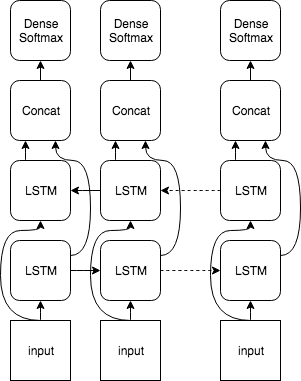
\includegraphics[width=0.5\linewidth]{Local}
	\end{center}
\end{figure}

\end{frame}

\begin{frame}
\frametitle{Символьные представление} 
\begin{table}[H]
		\caption{Пример данных в символьном представлении}
	
	\begin{small}
		\begin{center}
			\begin{tabular}{|c|l|}
				\hline
								Исходная фраза & поднятой руки было \\ \hline
				Фраза &{\usefont{T2A}{PTMono-TLF}{m}{n}ятой руки было} 
				\\ \hline
				Матрица ответа      &     {\usefont{T2A}{PTMono-TLF}{m}{n}11111111011111 }     \\ 
				& {\usefont{T2A}{PTMono-TLF}{m}{n}00000000100000 } \\ \hline
			\end{tabular}
		\end{center}
	\end{small}
\end{table}
\end{frame}

\begin{frame}
\frametitle{Результаты локальной символьной модели}
\begin{table}[H]	
	\begin{small}
		\begin{center}
			\begin{tabular}{|c|c|c|}
				\hline
				Число слогов & Gl Char & Loc Char \\ \hline
								\multicolumn{3}{|c|}{Все слова}                      \\ \hline
				
				2       &       0.983       &      0.961       \\ \hline
				3       &       0.977       &      0.940       \\ \hline
				4       &       0.976       &      0.947       \\ \hline
				5       &       0.977       &      0.960       \\ \hline
				6       &       0.973       &      0.958       \\ \hline
				7       &       0.955       &      0.924       \\ \hline
				8       &       0.923       &      0.866       \\ \hline
				9       &       0.952       &      0.809       \\ \hline
				AVG    &       0.979       &      0.952       \\ \hline
								\multicolumn{3}{|c|}{Омографы}                      \\ \hline
				
				2       &       0.810       &      0.839       \\ \hline
				3       &       0.844       &      0.774       \\ \hline
				4       &       0.847       &      0.787       \\ \hline
				AVG    &       0.819       &      0.821       \\ \hline
			\end{tabular}
		\end{center}
	\end{small}
\end{table}	
\end{frame}

\begin{frame}
\frametitle{Общие результаты}
\begin{table}[H]	
	\caption{Результаты на тестовой выборке}
	\begin{small}
		\begin{center}
			\begin{tabular}{|c|c|c|}
				\hline
				\diagbox{Модель}{Данные} & Символы & Слоги \\ \hline
				Локальная     & 0.952           &              \\ \hline
				Глобальная   &  0.979               &              \\ \hline
				Attention       &             &              \\ \hline
			\end{tabular}
		\end{center}
	\end{small}
\end{table}	

\begin{table}[H]	
		\caption{Результаты на омографах}
	\begin{small}
		\begin{center}
			\begin{tabular}{|c|c|c|}
				\hline
				\diagbox{Модель}{Данные} & Символы & Слоги \\ \hline
				Локальная      & 0.821             &              \\ \hline
				Глобальная    &0.819               &              \\ \hline
				Attention       &             &              \\ \hline
			\end{tabular}
		\end{center}
	\end{small}
\end{table}	


\end{frame}

\begin{frame}
\frametitle{Работа с предложениием}
\begin{table}[H]
	\caption{Пример данных для модели по предложениям}
	\begin{small}
		\begin{center}
			\begin{tabular}{|c|l|}
				\hline
				Исходная фраза & позволяет добиться того \\ \hline
				Фраза      & {\usefont{T2A}{PTMono-TLF}{m}{n}позволяет добиться того}  \\ \hline
				Матрица ответа & {\usefont{T2A}{PTMono-TLF}{m}{n}11111101111110111111110 } \\
				& {\usefont{T2A}{PTMono-TLF}{m}{n}00000010000001000000001 } \\ \hline
			\end{tabular}
		\end{center}
	\end{small}
	
	\label{table:local_sent_ex}
\end{table}

\end{frame}

\begin{frame}
\frametitle{Результаты локальной модели по предложениям}
\begin{table}[H]
\begin{small}
	\begin{center}
		\begin{tabular}{|c|c|c|}
			\hline
			Число слогов & Loc Char & Loc Sent \\ \hline
			\multicolumn{3}{|c|}{Все слова}                          \\ \hline
			2       &      0.961       &         0.897          \\ \hline
			3       &      0.940       &         0.891          \\ \hline
			4       &      0.947       &         0.902          \\ \hline
			5       &      0.960       &         0.927          \\ \hline
			6       &      0.958       &         0.925          \\ \hline
			7       &      0.924       &         0.898          \\ \hline
			8       &      0.866       &         0.855          \\ \hline
			9       &      0.809       &         0.647          \\ \hline
			AVG    &      0.952       &         0.898          \\ \hline
			\multicolumn{3}{|c|}{Омографы}                           \\ \hline
			2       &      0.839       &         0.831          \\ \hline
			3       &      0.774       &         0.754          \\ \hline
			4       &      0.787       &         0.775          \\ \hline
			AVG    &      0.821       &         0.812          \\ \hline
		\end{tabular}
	\end{center}
\end{small}

\label{table:local_sent}
\end{table}

\end{frame}


\begin{frame}
\frametitle{Слоговое представление}
\begin{itemize}
	\item Ударение падает только на гласные
	\item В каждом слоге 1 гласная
	\item \textbf{Правила разделения:} Всегда разделяем после гласной буквы, кроме
	\begin{itemize}
		\item последнего слога (за-бор)
		\item пары й + согласная (вой-на)
		\item  пары непарная согласная (р, л, м, н) и парная согласная (кар-тон)
	\end{itemize}
\end{itemize}
\begin{table}[H]
	\caption{Пример данных в слоговом представлении}
	\begin{small}
		\begin{center}
			\begin{tabular}{|c|l|}
				\hline
								Исходная фраза & позволяет добиться того \\ \hline
				Фраза &{\usefont{T2A}{PTMono-TLF}{m}{n}ля\_ет до\_би\_ться то\_го} 
				\\ \hline
				Матрица ответа      &     {\usefont{T2A}{PTMono-TLF}{m}{n} \ 1\ 1 1 1\ \  0\ \ \ \ 11 1\ \ 1 }     \\ 
				&  {\usefont{T2A}{PTMono-TLF}{m}{n}\ 0\ 0 0 0\ \  1\ \ \ \ 00 0\ \ 0} \\ \hline
			\end{tabular}
		\end{center}
	\end{small}
	
	\label{table:local_syl_ex}
\end{table}

\end{frame}

\begin{frame}
\frametitle{Результаты локальной слоговой модели} 
\begin{table}[H]	
	\begin{small}
		\begin{center}
			\begin{tabular}{|c|c|c|c|}
				\hline
				Число слогов & Gl Char & Loc Char & Loc Syl \\ \hline
							\multicolumn{4}{|c|}{Все слова}                          \\ \hline
				
				2       &       0.983       &      0.961       &      0.985      \\ \hline
				3       &       0.977       &      0.940       &      0.972      \\ \hline
				4       &       0.976       &      0.947       &      0.972      \\ \hline
				5       &       0.977       &      0.960       &      0.976      \\ \hline
				6       &       0.973       &      0.958       &      0.977      \\ \hline
				7       &       0.955       &      0.924       &      0.947      \\ \hline
				8       &       0.923       &      0.866       &      0.899      \\ \hline
				9       &       0.952       &      0.809       &      0.843      \\ \hline
				AVG    &       0.979       &      0.952       &      0.978      \\ \hline
							\multicolumn{4}{|c|}{Омографы}                          \\ \hline
				
				2       &       0.810       &      0.839       &      0.889      \\ \hline
				3       &       0.844       &      0.774       &      0.832      \\ \hline
				4       &       0.847       &      0.787       &      0.843      \\ \hline
				AVG    &       0.819       &      0.821       &      0.877      \\ \hline
			\end{tabular}
		\end{center}
	\end{small}
\end{table}	

\end{frame}

\begin{frame}
\frametitle{Общие результаты}
\begin{table}[H]	
	\caption{Результаты на тестовой выборке}
	\begin{small}
		\begin{center}
			\begin{tabular}{|c|c|c|}
				\hline
				\diagbox{Модель}{Данные} & Символы & Слоги \\ \hline
				       Локальная         &  0.952  & 0.978      \\ \hline
				       Глобальная        &  0.979  &       \\ \hline
				       Attention         &         &       \\ \hline
			\end{tabular}
		\end{center}
	\end{small}
\end{table}	

\begin{table}[H]	
\caption{Результаты на омографах}
\begin{small}
\begin{center}
\begin{tabular}{|c|c|c|}
	\hline
	\diagbox{Модель}{Данные} & Символы & Слоги \\ \hline
	       Локальная         &  0.821  &     0.877  \\ \hline
	       Глобальная        &  0.819  &       \\ \hline
	       Attention         &         &       \\ \hline
\end{tabular}
		\end{center}
	\end{small}
\end{table}	
\end{frame}




\subsection {Глобальная архитектура}
\begin{frame}
\frametitle{Глобальная архитектура} 
\begin{figure}[H]
	\begin{center}
		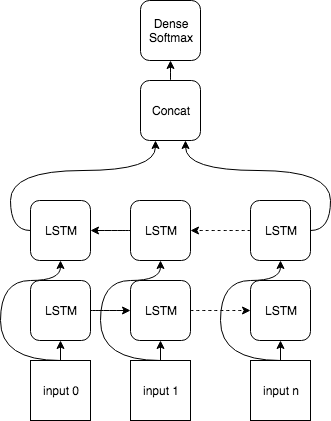
\includegraphics[width=0.5\linewidth]{Baseline}
	\end{center}
\end{figure}
\end{frame}
\begin{frame}
\frametitle{Результаты глобальной модели}
\begin{table}[H]	
	\begin{small}
		\begin{center}
			\begin{tabular}{|c|c|c| c|}
				\hline
				Число слогов & Gl Char & Loc Syl & Gl Syl \\ \hline
							\multicolumn{4}{|c|}{Все слова}                          \\ \hline
				
				2       &       0.983       &      0.985      & 0.985  \\ \hline
				3       &       0.977       &      0.972      &   0.978 \\ \hline
				4       &       0.976       &      0.972      &   0.977 \\ \hline
				5       &       0.977       &      0.976      &  0.977 \\ \hline
				6       &       0.973       &      0.977      &  0.970 \\ \hline
				7       &       0.955       &      0.947      &  0.945 \\ \hline
				8       &       0.923       &      0.899      &  0.895 \\ \hline
				9       &       0.952       &      0.843      & 0.849 \\ \hline
				AVG    &       0.979       &      0.978      & 0.981 \\ \hline
							\multicolumn{4}{|c|}{Омографы}                          \\ \hline
				
				2       &       0.810       &      0.889      & 0.893\\ \hline
				3       &       0.844       &      0.832      & 0.847\\ \hline
				4       &       0.847       &      0.843      & 0.852\\ \hline
				AVG    &       0.819       &      0.877      & 0.882 \\ \hline
			\end{tabular}
		\end{center}
	\end{small}
\end{table}	
\end{frame}

\begin{frame}
\frametitle{Общие результаты}
\begin{table}[H]	
	\caption{Результаты на тестовой выборке}
	\begin{small}
		\begin{center}
			\begin{tabular}{|c|c|c|}
				\hline
				\diagbox{Модель}{Данные} & Символы & Слоги \\ \hline
				Локальная         &  0.952  & 0.978      \\ \hline
				Глобальная        &  0.979  &   0.981    \\ \hline
				Attention         &         &       \\ \hline
			\end{tabular}
		\end{center}
	\end{small}
\end{table}	

\begin{table}[H]	
	\caption{Результаты на омографах}
	\begin{small}
		\begin{center}
			\begin{tabular}{|c|c|c|}
				\hline
				\diagbox{Модель}{Данные} & Символы & Слоги \\ \hline
				Локальная         &  0.821  &     0.877  \\ \hline
				Глобальная        &  0.819  &  0.882     \\ \hline
				Attention         &         &       \\ \hline
			\end{tabular}
		\end{center}
	\end{small}
\end{table}	
\end{frame}


\subsection{Модель с Attention}

\begin{frame}
\frametitle{Модель с Attention}

\begin{figure}[H]
	\begin{center}
		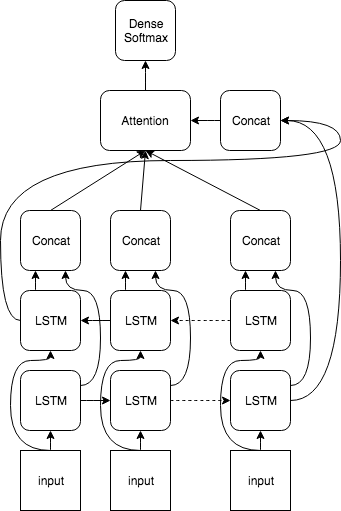
\includegraphics[width=0.48\linewidth]{Attention}
	\end{center}
\end{figure}


\end{frame}

\begin{frame}
\frametitle{Результаты модели с Attention}
\begin{table}[H]	
	\begin{small}
		\begin{center}
			\begin{tabular}{|c | c| c |}
				\hline
				
				Число слогов & Gl Syl & Att Syl \\ \hline
							\multicolumn{3}{|c|}{Все слова}                          \\ \hline
				
				2       & 0.985             & 0.989              \\ \hline
				3       & 0.978             & 0.982              \\ \hline
				4       & 0.977             & 0.979              \\ \hline
				5       & 0.977             & 0.980              \\ \hline
				6       & 0.970             & 0.969              \\ \hline
				7       & 0.945             & 0.936              \\ \hline
				8       & 0.895             & 0.867              \\ \hline
				9       & 0.849             & 0.747              \\ \hline
				AVG    & 0.981             & 0.985              \\ \hline
							\multicolumn{3}{|c|}{Все слова}                          \\ \hline
				
				2       & 0.893             & 0.900              \\ \hline
				3       & 0.847             & 0.869              \\ \hline
				4       & 0.852             & 0.846              \\ \hline
				AVG    & 0.882             & 0.889              \\ \hline
			\end{tabular}
		\end{center}
	\end{small}
	\label{table:global_att}
\end{table}


\end{frame}

\begin{frame}
\frametitle{Общие результаты}
\begin{table}[H]	
	\caption{Результаты на тестовой выборке}
	\begin{small}
		\begin{center}
			\begin{tabular}{|c|c|c|}
				\hline
				\diagbox{Модель}{Данные} & Символы & Слоги \\ \hline
				Локальная         &  0.952  & 0.978      \\ \hline
				Глобальная        &  0.979  &   0.981    \\ \hline
				Attention         &         &   0.985    \\ \hline
			\end{tabular}
		\end{center}
	\end{small}
\end{table}	

\begin{table}[H]	
	\caption{Результаты на омографах}
	\begin{small}
		\begin{center}
			\begin{tabular}{|c|c|c|}
				\hline
				\diagbox{Модель}{Данные} & Символы & Слоги \\ \hline
				Локальная         &  0.821  &     0.877  \\ \hline
				Глобальная        &  0.819  &  0.882     \\ \hline
				Attention         &         &  0.889     \\ \hline
			\end{tabular}
		\end{center}
	\end{small}
\end{table}	
\end{frame}

\begin{frame} 
\frametitle{Векторные представлениия слогов}
\begin{figure}[H]
	\begin{center}
		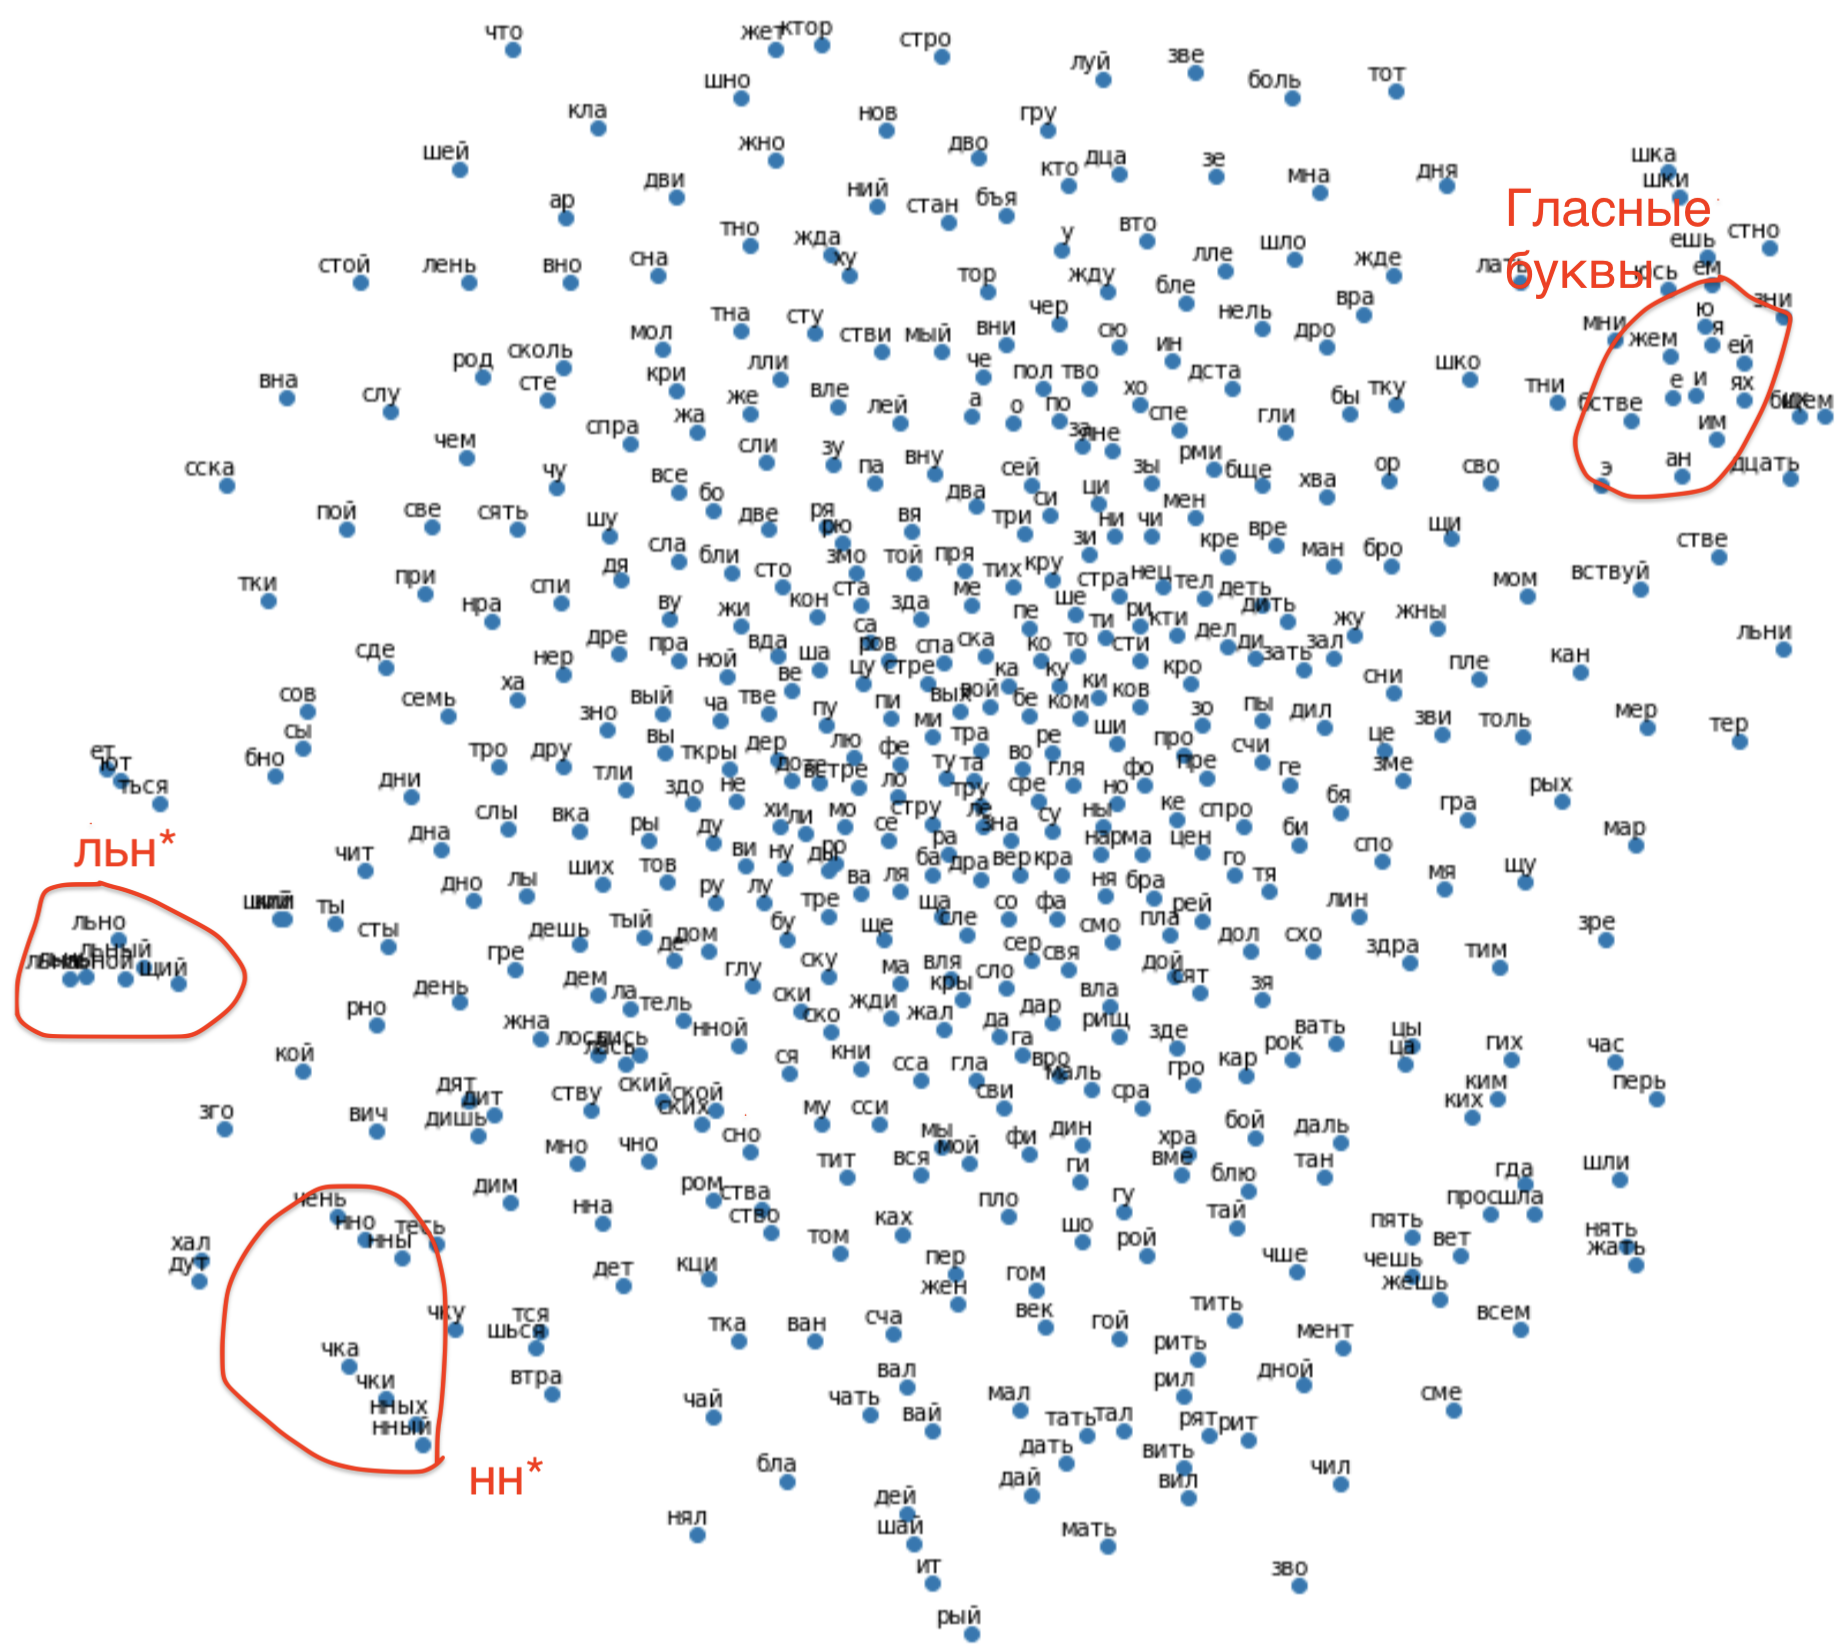
\includegraphics[width=0.8\linewidth]{Emb}
	\end{center}
\end{figure}

\end{frame}



\section{Анализ ошибок}
\subsection{Омографы}
\begin{frame}
\frametitle{Анализ ошибок: омографы}
\begin{itemize}
	\item 5\% в тексте
	\item 15\% среди ошибок
	\item Можно разделить на группы
	\begin{itemize}
		\item \textbf{Словоформы} \newline  рук\'{и} - р\'{у}ки \newline Accuracy score: 0.85
		\item \textbf{Разные части речи} \newline уж\'{е} - \'{у}же \newline Accuracy score: 0.94
		\item \textbf{Одна часть речи} \newline л\'{е}картсво - лек\'{а}рство \newline Accuracy score: 0.76	
\end{itemize}
	
\end{itemize}

\end{frame}
\subsection{Влияние контекста}
\begin{frame}
\frametitle{Анализ ошибок: влияние контекста}

\begin{table}[H]
	\caption{Зависимость от наличия контекста}
	\begin{small}
		\begin{center}
			\begin{tabular}{|c | c |}
				\hline
				Тип контекста  & Accuracy score \\ \hline
				Левый и правый & 0.986          \\ \hline
				Левый      & 0.984          \\ \hline
				Правый     & 0.977          \\ \hline
				Без контекста  & 0.976          \\ \hline
			\end{tabular}
		\end{center}
	\end{small}
\end{table}

\begin{table}[H]
	\caption{Распределение весов attention}
	\begin{small}
		\begin{center}
			\begin{tabular}{|c | c | c | c |}
				\hline
				Тип слов  & Левый контекст & Левый пробел & Слово\\ \hline
				Все слова & 0.008          & 0.294        & 0.551          \\ \hline
				Омографы  & 0.014          & 0.455        & 0.391           \\ \hline
				Тип слов  &  Правый контекст & Правый пробел & \\ \hline
				Все слова &  0.005   &     0.140         &   \\ \hline
				Омографы &  0.007  &      0.130         &    \\ \hline
			\end{tabular}
		\end{center}
	\end{small}
\end{table}

\end{frame}

\subsection{Новые слова}
\begin{frame}
\frametitle{Анализ ошибок: новые слова}
\begin{itemize}
	\item 10000 слов
	\item Accuracy score: 0.838
	\item Основные ошибки:
	\begin{itemize}
		\item Русские фамилии
		\item Заимствованные слова
		\item Многоосновные слова
	\end{itemize}
\end{itemize}
\end{frame}

\section{Active learning}
\begin{frame}
\frametitle{Active learning [\citenum{shen}]}
\begin{figure}[H]
	\caption{Результаты на тестовой выборке}
	\begin{center}
		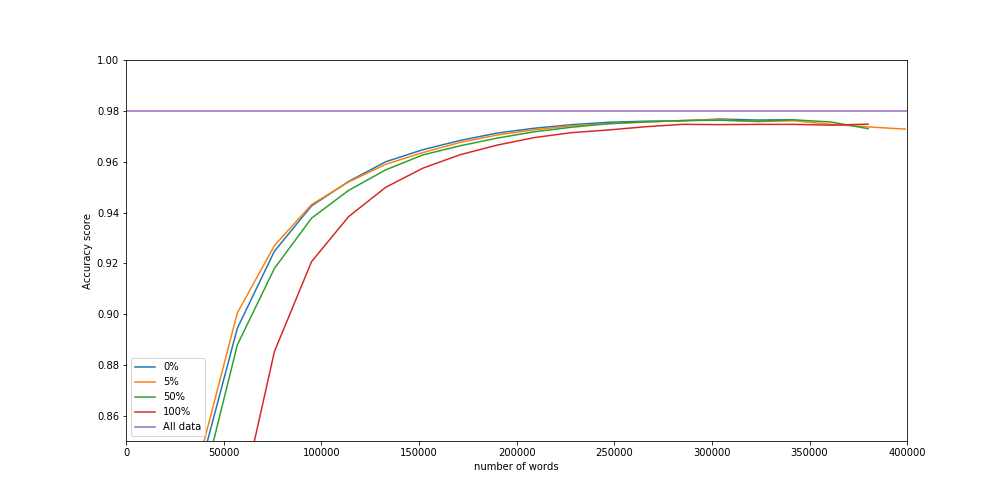
\includegraphics[width=1\linewidth]{All_scores}
	\end{center}
\end{figure}

\end{frame}

\begin{frame}
\frametitle{Active learning}
\begin{figure}[H]
	\caption{Результаты на омографах}
	\begin{center}
		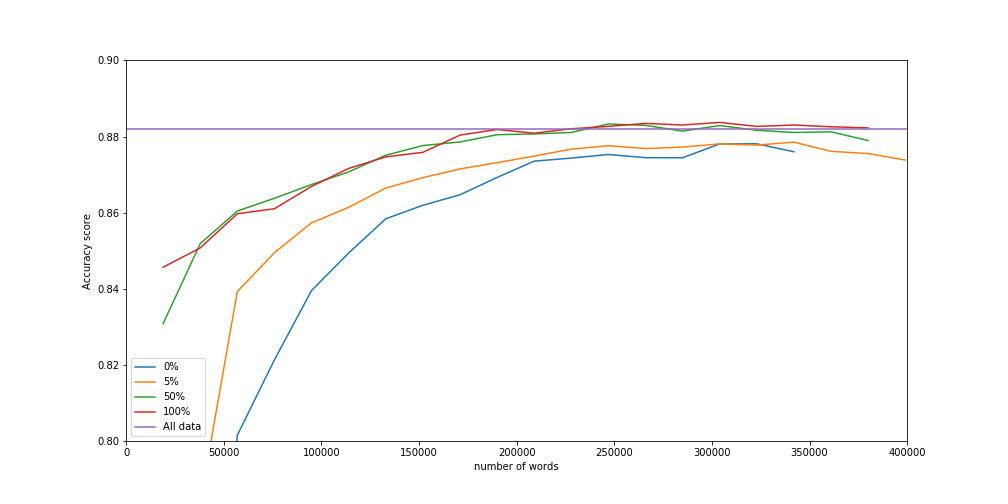
\includegraphics[width=1\linewidth]{Homo_scores}
	\end{center}
\end{figure}

\end{frame}

\begin{frame}
\frametitle{Active learning}
\begin{figure}[H]
	\caption{Доля омографов в новых данных}
	\begin{center}
		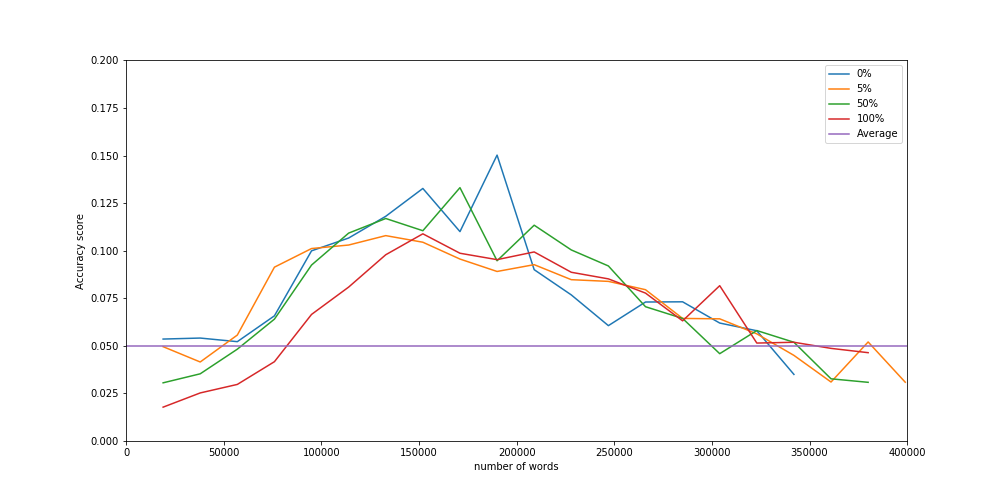
\includegraphics[width=1\linewidth]{Homo_perc}
	\end{center}
\end{figure}

\end{frame}



\section{Заключение}
\begin{frame}
\frametitle{Заключение}
\begin{itemize}
	\item Модель с attention показала наилучший результат(0.985)
	\item Слоговое представление данных позволяет улучшить результат с сохранением  архитектуры
	\item При помощи Active learning удалось снизить объем необходимых данных в 5 раз, сохранив при этом качество
\end{itemize}
\end{frame}
\begin{frame}
\begin{center}
	Спасибо за внимание
	\end{center}
\end{frame}
\begin{frame}
\frametitle{Список литературы }
{\footnotesize
	\bibliography{references}}
\end{frame}
\begin{frame}
\frametitle{Общие результаты}
\begin{table}[H]	
	\caption{Результаты на тестовой выборке}
	\begin{small}
		\begin{center}
			\begin{tabular}{|c|c|c|}
				\hline
				\diagbox{Модель}{Данные} & Символы & Слоги \\ \hline
				Локальная         &  0.952  & 0.978      \\ \hline
				Глобальная        &  0.979  &   0.981    \\ \hline
				Attention         &         &   0.985    \\ \hline
			\end{tabular}
		\end{center}
	\end{small}
\end{table}	

\begin{table}[H]	
	\caption{Результаты на омографах}
	\begin{small}
		\begin{center}
			\begin{tabular}{|c|c|c|}
				\hline
				\diagbox{Модель}{Данные} & Символы & Слоги \\ \hline
				Локальная         &  0.821  &     0.877  \\ \hline
				Глобальная        &  0.819  &  0.882     \\ \hline
				Attention         &         &  0.889     \\ \hline
			\end{tabular}
		\end{center}
	\end{small}
\end{table}	
\end{frame}

\begin{frame}
\frametitle{Сравнение результатов всех моделей}
\begin{table}[H]	
	\begin{small}
		\begin{center}
			\begin{tabular}{|c|c|c|c| c| c |}
				\hline
				Число слогов & Gl Char & Loc Char & Loc Syl & Gl syl & Att syl \\ \hline
							\multicolumn{6}{|c|}{Все слова}                          \\ \hline
				
				2       &       0.983       &      0.961       &      0.985      & 0.985             & 0.989              \\ \hline
				3       &       0.977       &      0.940       &      0.972      & 0.978             & 0.982              \\ \hline
				4       &       0.976       &      0.947       &      0.972      & 0.977             & 0.979              \\ \hline
				5       &       0.977       &      0.960       &      0.976      & 0.977             & 0.980              \\ \hline
				6       &       0.973       &      0.958       &      0.977      & 0.970             & 0.969              \\ \hline
				7       &       0.955       &      0.924       &      0.947      & 0.945             & 0.936              \\ \hline
				8       &       0.923       &      0.866       &      0.899      & 0.895             & 0.867              \\ \hline
				9       &       0.952       &      0.809       &      0.843      & 0.849             & 0.747              \\ \hline
				AVG    &       0.979       &      0.952       &      0.978      & 0.981             & 0.985              \\ \hline
							\multicolumn{6}{|c|}{Омографы}                          \\ \hline
				
				2       &       0.810       &      0.839       &      0.889      & 0.893             & 0.900              \\ \hline
				3       &       0.844       &      0.774       &      0.832      & 0.847             & 0.869              \\ \hline
				4       &       0.847       &      0.787       &      0.843      & 0.852             & 0.846              \\ \hline
				AVG    &       0.819       &      0.821       &      0.877      & 0.882             & 0.889              \\ \hline
			\end{tabular}
		\end{center}
	\end{small}
\end{table}	

\end{frame}

\end{document}

